\setcounter{chapter}{17} % Chapter 18
\chapter{Constructing New Vector Spaces Out of Old Ones}

\setcounter{section}{0}
\section{The Homomorphism Space, The Dual Space And The Dual Map}

\subsection{The Homomorphism Space}

\begin{proposition}[The Vector Space Structure of the Homomorphism Space]
  Let $V$ and $W$ be two vector spaces over $K$. Then, $\Hom(V,W)$ has the structure of a vector space over $K$, if we endow it with the following operations:
  \begin{itemize}
    \item For all $T_1, T_2 \in \Hom(V,W)$, $(T_1 + T_2)(v) := T_1(v) + T_2(v)$ for all $v \in V$.
    \item For all $T \in \Hom(V,W)$ and $\alpha \in K$, $(\alpha \cdot T)(v) := \alpha \cdot T(v)$ for all $v \in V$.
  \end{itemize}
\end{proposition}

\begin{proof}
  We claim that $T_1 + T_2 \in \Hom(V,W)$, meaning $T_1 + T_2$ is a linear map. Indeed, for a scalar $a$ and a vector $v$, we have
  \begin{align*}
    (T_1 + T_2)(a \cdot v) &= T_1(a \cdot v) + T_2(a \cdot v) = a \cdot T_1(v) + a \cdot T_2(v) \\
    &= a \cdot (T_1(v) + T_2(v)) = a \cdot (T_1 + T_2)(v),
  \end{align*}
  and for vectors $v_1, v_2$, we have
  \begin{align*}
    (T_1 + T_2)(v_1 + v_2) &= T_1(v_1 + v_2) + T_2(v_1 + v_2) = T_1(v_1) + T_1(v_2) + T_2(v_1) + T_2(v_2) \\
    &= (T_1 + T_2)(v_1) + (T_1 + T_2)(v_2).
  \end{align*}
  Consequently, $T_1 + T_2$ is a linear map. The proof that $\alpha \cdot T$ is linear is analogous.

  So far, we have defined $+ \colon \Hom(V,W) \times \Hom(V,W) \to \Hom(V,W)$ and $\cdot \colon K \times \Hom(V,W) \to \Hom(V,W)$.

  Regarding the neutral element, the map $0 \colon V \to W$ defined by $v \mapsto 0$ for all $v \in V$ is linear. We claim that $0 + T = T$. Indeed,
  $$(0 + T)(v) = 0(v) + T(v) = 0 + T(v) = T(v)$$
  for all $v \in V$. Similarly, one shows that $T + \mathcal{O} = T$.
  for all $v \in V$. Similarly, one shows that $T + 0 = T$.
\end{proof}

\begin{exercise}
  Complete the proof that $\Hom(V,W)$ is a vector space by checking that it satisfies all the axioms of a vector space, using the zero map $0 \colon V \to W$ as the additive identity.
\end{exercise}

For example, consider the distributivity axiom. For all $\alpha \in K$ and $T_1, T_2 \in \Hom(V,W)$, we have $\alpha \cdot (T_1 + T_2) = \alpha \cdot T_1 + \alpha \cdot T_2$. Indeed, for $v \in V$,
\begin{align*}
  (\alpha \cdot (T_1 + T_2))(v) &= \alpha \cdot (T_1 + T_2)(v) = \alpha(T_1(v) + T_2(v)) \\
  &= \alpha \cdot T_1(v) + \alpha \cdot T_2(v) = (\alpha \cdot T_1)(v) + (\alpha \cdot T_2)(v) \\
  &= (\alpha \cdot T_1 + \alpha \cdot T_2)(v).
\end{align*}
Therefore, $\alpha \cdot (T_1 + T_2) = \alpha \cdot T_1 + \alpha \cdot T_2$.

\begin{theorem}[The Canonical Isomorphism to Matrix Space]
  Let $V$ and $W$ be finite-dimensional vector spaces over $K$, let $\mathcal{B} = (v_1, \dots, v_n)$ be a basis for $V$, and let $\mathcal{C} = (w_1, \dots, w_m)$ be a basis for $W$. Then, $\Psi_{\mathcal{C}}^{\mathcal{B}} \colon \Hom(V,W) \to M_{m \times n}(K)$, defined by
  $$\Psi_{\mathcal{C}}^{\mathcal{B}}(T) := [T]_{\mathcal{C}}^{\mathcal{B}} = \begin{pmatrix} | & & | \\ [T(v_1)]_{\mathcal{C}} & \dots & [T(v_n)]_{\mathcal{C}} \\ | & & | \end{pmatrix},$$
  is a linear map, and moreover, an isomorphism.
\end{theorem}

\begin{proof}
  Recall that $T_{[T]_{\mathcal{C}}^{\mathcal{B}}} = \Phi_{\mathcal{C}} \circ T \circ \Phi_{\mathcal{B}}^{-1}$. Recall also that $\Phi_{\mathcal{B}}(v) = [v]_{\mathcal{B}} \in K^n$ for all $v \in V$. Furthermore, $\Phi_{\mathcal{C}}(w) = [w]_{\mathcal{C}} \in K^m$ for all $w \in W$. We have
  $$\Phi_{\mathcal{B}}^{-1} \begin{pmatrix} a_1 \\ \vdots \\ a_n \end{pmatrix} = a_1 v_1 + \dots + a_n v_n, \quad \Phi_{\mathcal{C}}^{-1} \begin{pmatrix} b_1 \\ \vdots \\ b_m \end{pmatrix} = b_1 w_1 + \dots + b_m w_m.$$

  We claim that the map $\Psi_{\mathcal{C}}^{\mathcal{B}}$ is bijective. Indeed, define $\Theta \colon M_{m \times n}(K) \to \Hom(V,W)$ by $\Theta(A) := \Phi_{\mathcal{C}}^{-1} \circ T_A \circ \Phi_{\mathcal{B}} \in \Hom(V,W)$ for $A \in M_{m \times n}(K)$. We have:
  \begin{align*}
    \Psi_{\mathcal{C}}^{\mathcal{B}} \circ \Theta(A) &= \Psi_{\mathcal{C}}^{\mathcal{B}}(\Phi_{\mathcal{C}}^{-1} \circ T_A \circ \Phi_{\mathcal{B}}) \\
    &= \left( [\Phi_{\mathcal{C}}^{-1} \circ T_A \circ \Phi_{\mathcal{B}}(v_1)]_{\mathcal{C}} \dots [\Phi_{\mathcal{C}}^{-1} \circ T_A \circ \Phi_{\mathcal{B}}(v_n)]_{\mathcal{C}} \right) \\
    &= \begin{pmatrix} | & & | \\ T_A \Phi_{\mathcal{B}}(v_1) & \dots & T_A \Phi_{\mathcal{B}}(v_n) \\ | & & | \end{pmatrix} \\
    &= \begin{pmatrix} | & & | \\ T_A(e_1) & \dots & T_A(e_n) \\ | & & | \end{pmatrix} = A.
  \end{align*}
  This uses the facts that $[\Phi_{\mathcal{C}}^{-1}(b)]_{\mathcal{C}} = b$ for all $b \in K^m$, and $\Phi_{\mathcal{B}}(v_k) = e_k$. This proves that $\Psi_{\mathcal{C}}^{\mathcal{B}} \circ \Theta = \id_{M_{m \times n}(K)}$.

  Now, by definition, $\Theta \circ \Psi_{\mathcal{C}}^{\mathcal{B}}(T) = \Phi_{\mathcal{C}}^{-1} \circ T_{\Psi_{\mathcal{C}}^{\mathcal{B}}(T)} \circ \Phi_{\mathcal{B}} = \Phi_{\mathcal{C}}^{-1} \circ T_{[T]_{\mathcal{C}}^{\mathcal{B}}} \circ \Phi_{\mathcal{B}} = T$. This shows that $\Theta \circ \Psi_{\mathcal{C}}^{\mathcal{B}} = \id_{\Hom(V,W)}$. Therefore, $\Psi_{\mathcal{C}}^{\mathcal{B}}$ is bijective.

  It remains to prove that $\Psi_{\mathcal{C}}^{\mathcal{B}}$ is linear. Indeed, let $\alpha \in K$, and let $T \in \Hom(V,W)$. Then,
  \begin{align*}
    \Psi_{\mathcal{C}}^{\mathcal{B}}(\alpha \cdot T) &= \left( [(\alpha T)(v_1)]_{\mathcal{C}} \dots [(\alpha T)(v_n)]_{\mathcal{C}} \right) \\
    &= \left( [\alpha T(v_1)]_{\mathcal{C}} \dots [\alpha T(v_n)]_{\mathcal{C}} \right) \\
    &= \left( \alpha [T(v_1)]_{\mathcal{C}} \dots \alpha [T(v_n)]_{\mathcal{C}} \right) \\
    &= \alpha \cdot \begin{pmatrix} | & & | \\ [T(v_1)]_{\mathcal{C}} & \dots & [T(v_n)]_{\mathcal{C}} \\ | & & | \end{pmatrix} \\
    &= \alpha \cdot \Psi_{\mathcal{C}}^{\mathcal{B}}(T).
  \end{align*}
  Similarly, one shows that $\Psi_{\mathcal{C}}^{\mathcal{B}}(T_1 + T_2) = \Psi_{\mathcal{C}}^{\mathcal{B}}(T_1) + \Psi_{\mathcal{C}}^{\mathcal{B}}(T_2)$.
\end{proof}

\begin{corollary}[Dimensionality of the Homomorphism Space]
  If $V$ and $W$ are finite-dimensional vector spaces, then so is $\Hom(V,W)$, and $\dim \Hom(V,W) = \dim V \cdot \dim W$.
\end{corollary}

\begin{proof}
  Put $n := \dim V$ and $m := \dim W$. By the previous theorem, we have $\Hom(V,W) \cong M_{m \times n}(K)$, which implies that $\Hom(V,W)$ is finite-dimensional. Moreover, $\dim \Hom(V,W) = \dim M_{m \times n}(K) = m \cdot n$.
\end{proof}

\subsection{Rings}
\begin{example}
  \begin{enumerate}
    \item Every field $K$ is also a commutative ring.
    \item $\mathbb{Z}$ is a commutative ring.
    \item $M_{n \times n}(K)$ is a ring, where $A \cdot B$ is matrix multiplication, and the unity is $I_n$. Clearly, it is not commutative.
  \end{enumerate}
\end{example}

\begin{corollary}[The Ring of Endomorphisms]
  Let $V$ be a vector space over $K$. Then, $\End(V) := \Hom(V,V)$ is a ring with a unity. This ring is, in general, not commutative. The multiplication in $\End(V)$ is given by composition $T_1 \cdot T_2 := T_1 \circ T_2$ for all $T_1, T_2 \in \Hom(V,V)$, and the unity is $\id_V$. Moreover, if $V$ is finite-dimensional with $\dim V = n$, and $\mathcal{B} = (w_1, \dots, w_n)$ is a basis for $V$, then $\Psi_{\mathcal{B}}^{\mathcal{B}} \colon \Hom(V,V) \to M_{n \times n}(K)$ is an isomorphism of rings.
\end{corollary}

\begin{proof}[Proof (sketch)]
  The multiplication $T_1 \cdot T_2 := T_1 \circ T_2$ is associative, since $(T_1 \cdot T_2) \cdot T_3 = (T_1 \circ T_2) \circ T_3 = T_1 \circ (T_2 \circ T_3) = T_1 \cdot (T_2 \cdot T_3)$. Also, $T \cdot \id_V = T \circ \id_V = T$, and $\id_V \cdot T = \id_V \circ T = T$. Furthermore, $T \cdot (T_1 + T_2) = T \circ (T_1 + T_2) = T \circ T_1 + T \circ T_2$.

  Now, if $V$ is finite-dimensional, and $\mathcal{B}$ is a basis for $V$, then
  $$\Psi_{\mathcal{B}}^{\mathcal{B}}(T_1 \circ T_2) = [T_1 \circ T_2]_{\mathcal{B}}^{\mathcal{B}} = [T_1]_{\mathcal{B}}^{\mathcal{B}} \cdot [T_2]_{\mathcal{B}}^{\mathcal{B}} = \Psi_{\mathcal{B}}^{\mathcal{B}}(T_1) \cdot \Psi_{\mathcal{B}}^{\mathcal{B}}(T_2)$$
  via matrix multiplication.
\end{proof}

\subsection{The Dual Space}
An important special case of $\Hom(V,W)$ is when $W=K$.

\begin{definition}[The Dual Space and Linear Functionals]
  Let $V$ be a vector space over $K$. The dual space of $V$ is defined to be the vector space $V^* := \Hom(V,K)$. The elements of $V^*$ are linear maps $l \colon V \to K$, and are sometimes called functionals.
\end{definition}

\begin{corollary}[Dimensionality of the Dual Space]
  Let $V$ be a finite-dimensional vector space over $K$. Then, $\dim V^* = \dim V$.
\end{corollary}

\begin{proof}
  We have $\dim V^* = \dim \Hom(V,K) = \dim V \cdot \dim K = \dim V \cdot 1 = \dim V$.
\end{proof}

Let $V = K_{\text{col}}^n$. Then, we can identify $V^*$ with $K_{\text{row}}^n$ as follows: If $l \in K_{\text{row}}^n$, then $l$ defines a functional $f_l \colon K_{\text{col}}^n \to K$ by $f_l(v) := l \cdot v \in M_{1 \times 1}(K) \cong K$. The map $D \colon K_{\text{row}}^n \to (K_{\text{col}}^n)^*$ defined by $D(l) := f_l$ is a linear map, and therefore, it is an isomorphism.

Let $V$ be a finite-dimensional vector space over $K$, and let $\mathcal{B} = (v_1, \dots, v_n)$ be a basis for $V$. For $1 \leq i \leq n$, define a functional $v_i^* \in V^*$ as follows: $v_i^*(v_j) := \delta_{ij}$. This means that $v_i^*(v_i) = 1$, and $v_i^*(v_j) = 0$ for all $j \neq i$. Since $v_1, \dots, v_n$ form a basis for $V$, our definition determines uniquely a well-defined functional $v_i^* \colon V \to K$.

\begin{lemma}[Construction of the Dual Basis]
  The elements $v_1^*, \dots, v_n^* \in V^*$ form a basis for $V^*$. This basis is called the dual basis to $\mathcal{B}$. We denote this basis by $\mathcal{B}^* = (v_1^*, \dots, v_n^*)$. Moreover, for all $l \in V^*$, $l = \sum_{i=1}^n l(v_i) \cdot v_i^*$.
\end{lemma}

\begin{proof}
  Let $l \in V^*$. We claim that $l = \sum_{i=1}^n l(v_i) \cdot v_i^*$, or in other words, we claim that $l(v) = \sum_{i=1}^n l(v_i) \cdot v_i^*(v)$. Indeed, both sides of the equation are linear maps $V \to K$, and therefore, it is enough to check that it holds for $v = v_1, v = v_2, \dots, v = v_n$, because $v_1, \dots, v_n$ form a basis for $V$. And indeed, for $v = v_k$, we have:
  $$\sum_{i=1}^n l(v_i) \cdot v_i^*(v_k) = \sum_{i=1}^n l(v_i) \cdot \delta_{ik} = l(v_k).$$
  The claim just proven shows that $v_1^*, \dots, v_n^*$ span $V^*$. Since $\dim V^* = \dim V = n$, it follows that $v_1^*, \dots, v_n^*$ form a basis for $V^*$.
\end{proof}

\begin{question}Let $V$ be a finite-dimensional vector space over $K$, and let $\mathcal{B}$ and $\mathcal{C}$ be two bases for $V$. $\mathcal{B}^*$ and $\mathcal{C}^*$ are two bases for $V^*$. What is the relation between $[\id_{V^*}]_{\mathcal{B}^*}^{\mathcal{C}^*}$ and $[\id_V]_{\mathcal{B}}^{\mathcal{C}}$?
\end{question}

\begin{proposition}[Dual Change of Basis and Transposition]
  The relationship between transition matrices in the dual space and the primal space is characterized by transposition and inversion. Specifically, the transition matrix between dual bases $\mathcal{C}^*$ and $\mathcal{B}^*$ is the transpose of the inverse transition matrix between the original bases $\mathcal{C}$ and $\mathcal{B}$:
  \[
  [\id_{V^*}]_{\mathcal{B}^*}^{\mathcal{C}^*} = \left( [\id_V]_{\mathcal{C}}^{\mathcal{B}} \right)^T = \left( \left( [\id_V]_{\mathcal{B}}^{\mathcal{C}} \right)^{-1} \right)^T.
  \]
  Thus, the coordinate transformation in the dual space corresponds to the transpose of the inverse transformation in the primal space.
\end{proposition}

\begin{proof}
  Let $\mathcal{B} = (v_1, \dots, v_n)$, and let $\mathcal{C} = (w_1, \dots, w_n)$. We have $A := [\id_V]_{\mathcal{C}}^{\mathcal{B}} = \begin{pmatrix} | & & | \\ [v_1]_{\mathcal{C}} & \dots & [v_n]_{\mathcal{C}} \\ | & & | \end{pmatrix}$. Write $A = (a_{ij})$. By definition, $v_i = \sum_{k=1}^n a_{ki} w_k$.
  Let $\mathcal{C}^* = (w_1^*, \dots, w_n^*)$ be the dual basis of $\mathcal{C}$. We apply the previous lemma to $l = w_j^*$ and the basis $\mathcal{B}$:
  $$w_j^* = \sum_{i=1}^n w_j^*(v_i) \cdot v_i^* = \sum_{i=1}^n w_j^*\left(\sum_{k=1}^n a_{ki} w_k\right) \cdot v_i^* = \sum_{i=1}^n a_{ji} v_i^*.$$
  Here, only $k = j$ remains from the inner sum. This implies that $[\id_{V^*}]_{\mathcal{B}^*}^{\mathcal{C}^*} = A^T = ([\id_V]_{\mathcal{C}}^{\mathcal{B}})^T$.
\end{proof}

\subsection{The Dual Map}
\begin{lemma}[Definition of the Dual Map]
  Let $V$ and $W$ be vector spaces over $K$, and let $T \colon V \to W$ be a linear map. Define a new map $T^* \colon W^* \to V^*$ by $T^*(l) := l \circ T$ for all $l \in W^*$. Then, $T^*$ is a linear map. It is called the dual map to $T$.
\end{lemma}

\begin{proof}
  Let $l \in W^*$, meaning $l \colon W \to K$ is linear. Clearly, $l \circ T \colon V \to K$ is a linear map because both $T$ and $l$ are linear, so $T^*(l) := l \circ T \in V^*$. This shows that $T^* \colon W^* \to V^*$ has its target indeed in $V^*$, as claimed.

  We will show now that $T^*$ is a linear map. Let $l \in W^*$, and let $\alpha \in K$. We have that $T^*(\alpha l) \in V^*$ is the map:
  $$T^*(\alpha l)(v) = ((\alpha l) \circ T)(v) = (\alpha l)(T(v)) = \alpha l(T(v)) = \alpha \cdot (l \circ T)(v) = \alpha (T^* l)(v).$$
  So, $T^*(\alpha l) = \alpha \cdot T^*(l)$. Similarly, one shows that $T^*(l_1 + l_2) = T^*(l_1) + T^*(l_2)$.
\end{proof}

\begin{proposition}[Functoriality and Composition of Duals]
  Let $U, V, W$ be vector spaces over $K$, and let $T \colon V \to W$ and $S \colon W \to U$ be linear maps. Consider the dual maps $T^* \colon W^* \to V^*$ and $S^* \colon U^* \to W^*$. Then, $(S \circ T)^* = T^* \circ S^*$.
\end{proposition}

\begin{proof}
  Exercise.
\end{proof}

\begin{exercise}
  Let $V$ be a vector space over $K$. Show that:
  \begin{enumerate}
    \item $(\id_V)^* = \id_{V^*}$.
    \item $(0 \colon V \to V)^* = (0 \colon V^* \to V^*)$.
  \end{enumerate}
\end{exercise}

In summary, applying $(-)^*$, or $\Hom(-,K)$, takes every vector space $V$ and gives us a new vector space $V^*$. It also takes any linear map $T \colon V \to W$ and gives us a new map $T^*$ between the duals of $V$ and $W$, but the arrow is reversed: $T^* \colon W^* \to V^*$. This is an example of a contravariant functor.

\begin{lemma}[Transposition of the Representation Matrix]
  Let $S \colon V \to W$ be a linear map between two finite-dimensional vector spaces $V$ and $W$ over $K$. Let $\mathcal{B}$ be a basis for $V$, and let $\mathcal{C}$ be a basis for $W$. Consider $S^* \colon W^* \to V^*$ and the bases $\mathcal{C}^*, \mathcal{B}^*$ for $W^*, V^*$, respectively. Then, $[S^*]_{\mathcal{B}^*}^{\mathcal{C}^*} = ([S]_{\mathcal{C}}^{\mathcal{B}})^T$.
\end{lemma}

\begin{proof}
  Write $\mathcal{B} = (v_1, \dots, v_n)$, $\mathcal{C} = (w_1, \dots, w_m)$, and $A := [S]_{\mathcal{C}}^{\mathcal{B}} = (a_{ij})$. $A$ satisfies $S(v_j) = \sum_{i=1}^m a_{ij} w_i$. Now, for $w_j^* \in \mathcal{C}^*$, we have
  $$S^*(w_j^*) = w_j^* \circ S = \sum_{i=1}^n (w_j^* \circ S)(v_i) \cdot v_i^* = \sum_{i=1}^n w_j^*(S(v_i)) \cdot v_i^*,$$
  where the second equality follows from the Lemma on the Dual Basis. Substituting $S(v_i)$, we get
  $$= \sum_{i=1}^n w_j^*\left(\sum_{k=1}^m a_{ki} w_k\right) \cdot v_i^* = \sum_{i=1}^n a_{ji} v_i^*.$$
  The coordinates of $S^*(w_j^*)$ in the basis $\mathcal{B}^* = (v_1^*, \dots, v_n^*)$ are $\left(\begin{smallmatrix} a_{j1} \\ \vdots \\ a_{jn} \end{smallmatrix}\right)$, which corresponds to row $j$ in $A$, represented as a column (i.e., column $j$ in $A^T$).
\end{proof}

\subsection{Reflexivity}
Let $V$ be a vector space over $K$. We have $V^*$, but also $V^{**} := (V^*)^*$, obtained by applying the ``dual'' operation one more time to $V^*$. $V^{**}$ is sometimes called the bidual space of $V$. Is there any relation between $V^{**}$ and $V$?

\begin{theorem}[The Canonical Isomorphism to the Bidual Space]
  Let $V$ be a finite-dimensional vector space over $K$. Then, there is a canonical isomorphism $\tau \colon V \to (V^*)^*$ given by: for $v \in V$, $\tau(v) \colon V^* \to K$ is the map $\tau(v)(l) := l(v)$ for all $l \in V^*$.
\end{theorem}

\begin{remark}
  The map $\tau \colon V \to (V^*)^*$ exists and is defined in the same way as above regardless of $V$ being finite- or infinite-dimensional. Moreover, $\tau$ is always injective. However, when $V$ is infinite-dimensional, $\tau$ fails to be surjective.
\end{remark}

\begin{proof}
  We claim that $\tau$ is a linear map. Indeed, if $v \in V$ and $\alpha \in K$, we have
  \begin{align*}
    \tau(\alpha v) &= (V^* \ni l \mapsto l(\alpha v) \in K) \\
    &= (V^* \ni l \mapsto \alpha l(v) \in K) \\
    &= \alpha \cdot (V^* \ni l \mapsto l(v) \in K) = \alpha \tau(v).
  \end{align*}
  Similarly, one shows that $\tau(v' + v'') = \tau(v') + \tau(v'')$.

  We now claim that $\tau$ is injective. To see this, we will show that $\ker(\tau) = 0$. Indeed, let $v \in \ker(\tau)$, meaning $\tau(v) = 0$. Then, $l(v) = 0$ for all $l \in V^*$. Choose a basis $\mathcal{B} = (v_1, \dots, v_n)$ for $V$. Write $v = c_1 v_1 + \dots + c_n v_n$. Apply $v_k^*$ to $v$, and we obtain $v_k^*(c_1 v_1 + \dots + c_n v_n) = 0$. But $v_k^*(c_1 v_1 + \dots + c_n v_n) = c_k$. Therefore, $c_k = 0$, and this holds for $1 \leq k \leq n$, which implies that $v = 0$. This proves that $\tau$ is injective.

  To finish the proof, note that $\dim(V^*)^* = \dim V^* = \dim V$. So, since $\tau \colon V \to (V^*)^*$ is injective, it must be an isomorphism.
\end{proof}

\begin{remark}
  The previous theorem is not true for infinite-dimensional vector spaces. More specifically, $\tau \colon V \to (V^*)^*$ is injective, but not surjective. In fact, when $V$ is infinite-dimensional, $(V^*)^*$ is not isomorphic to $V$.
\end{remark}

\subsection{Naturality}
The map $\tau \colon V \to (V^*)^*$ exists for every space $V$, and it is defined in the same way. To distinguish $\tau$'s for different spaces, we denote it by $\tau_V \colon V \to (V^*)^*$. Let $V$ and $W$ be two vector spaces over $K$. Then, for any linear map $T \colon V \to W$, we have the following naturality condition, represented by a commutative diagram:

\begin{center}
  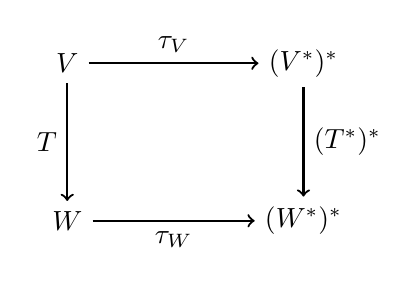
\begin{tikzpicture}[node distance=3cm, auto, thick]
    \node (V) {$V$};
    \node (Vdual) [right of=V] {$(V^*)^*$};
    \node (W) [below of=V, node distance=2cm] {$W$};
    \node (Wdual) [right of=W] {$(W^*)^*$};

    \draw[->] (V) to node {$\tau_V$} (Vdual);
    \draw[->] (V) to node[swap] {$T$} (W);
    \draw[->] (W) to node[swap] {$\tau_W$} (Wdual);
    \draw[->] (Vdual) to node {$(T^*)^*$} (Wdual);
  \end{tikzpicture}
\end{center}

\begin{exercise}
  Let $V$ be a finite-dimensional vector space over $K$, and let $\mathcal{B} = (v_1, \dots, v_n)$ be a basis for $V$. Let $\mathcal{B}^* = (v_1^*, \dots, v_n^*)$ be the dual basis, and let $(\mathcal{B}^*)^* = ((v_1^*)^*, \dots, (v_n^*)^*)$ be the basis for $(V^*)^*$ which is dual to $\mathcal{B}^*$. Show that $\tau(\mathcal{B}) = (\mathcal{B}^*)^*$, meaning $\tau(v_i) = (v_i^*)^*$ for all $1 \leq i \leq n$.
\end{exercise}

\setcounter{section}{1}
\section{Direct Sums}

\subsection{The External Direct Sum}

\begin{proposition}[Vector Space Structure of the Cartesian Product]
  Let $V$ and $W$ be two vector spaces over $K$. Then, the Cartesian product $V \times W$ becomes a vector space over $K$, provided we endow it with the following operations:
  \begin{itemize}
    \item $(v_1, w_1) + (v_2, w_2) := (v_1 + v_2, w_1 + w_2)$ for all $(v_1, w_1), (v_2, w_2) \in V \times W$.
    \item $\alpha \cdot (v, w) := (\alpha v, \alpha w)$ for all $\alpha \in K$ and $(v, w) \in V \times W$.
  \end{itemize}
  The zero element of this space is given by $0_{V \times W} := (0_V, 0_W)$. This new vector space $V \times W$ is usually denoted by $V \oplus W$ and is called the direct sum of $V$ and $W$.
\end{proposition}

\begin{proof}
  Exercise. One must verify that all vector space axioms are satisfied under these componentwise operations.
\end{proof}

\begin{remark}[Canonical Maps associated with Direct Sums]
  The direct sum $V \oplus W$ is naturally equipped with several canonical linear maps:
  \begin{enumerate}
    \item \textbf{Canonical Embeddings}:
    \begin{itemize}
      \item $i_V \colon V \to V \oplus W$ defined by $i_V(v) := (v, 0)$.
      \item $i_W \colon W \to V \oplus W$ defined by $i_W(w) := (0, w)$.
    \end{itemize}
    \item \textbf{Canonical Projections}:
    \begin{itemize}
      \item $p_V \colon V \oplus W \to V$ defined by $p_V(v, w) := v$.
      \item $p_W \colon V \oplus W \to W$ defined by $p_W(v, w) := w$.
    \end{itemize}
  \end{enumerate}
  Clearly, all these maps are linear. Furthermore, the projections $p_V$ and $p_W$ are surjective, while the embeddings $i_V$ and $i_W$ are injective. By virtue of these embeddings, we can often identify $V$ and $W$ as subspaces of $V \oplus W$ through the identifications $v \leftrightarrow (v, 0)$ and $w \leftrightarrow (0, w)$.
\end{remark}

\subsection{Internal Direct Sums and Complements}

\begin{proposition}[Isomorphism to a Complementary Subspace]
  Let $V$ be a vector space over $K$, and let $U \subseteq V$ be a subspace. Suppose $U' \subseteq V$ is another subspace that acts as a complement of $U$ in $V$, which implies that $U + U' = V$ and $U \cap U' = \{0\}$. Then, the map
  \[
  \varphi \colon U \oplus U' \to V, \quad \varphi(u, u') := u + u'
  \]
  is a linear isomorphism.
\end{proposition}

\begin{proof}
  The linearity of $\varphi$ follows immediately from the definitions of the operations in $U \oplus U'$ and the linearity of addition in $V$.

  To establish injectivity, suppose $\varphi(u, u') = 0$, which implies $u + u' = 0$, and therefore $u = -u'$. Since $u \in U$ and $u' \in U'$, it follows that $u = -u' \in U \cap U'$. However, as $U'$ is a complement of $U$, we have $U \cap U' = \{0\}$ by definition. Consequently, $u = u' = 0$, which shows that $\ker(\varphi) = \{0_{U \oplus U'}\}$. Thus, $\varphi$ is injective.

  Regarding surjectivity, we observe that since $U'$ is a complement of $U$ in $V$, we have $U + U' = V$ by definition. Thus, for any $v \in V$, there exist $u \in U$ and $u' \in U'$ such that $u + u' = v$. This implies $\varphi(u, u') = v$, and therefore $\operatorname{Im}(\varphi) = V$. This proves that $\varphi$ is surjective, and consequently, an isomorphism.
\end{proof}

\begin{remark}
  While $U \oplus U'$ is formally a different vector space from $V$, the existence of the canonical isomorphism $\varphi$ allows us to treat $V$ as the direct sum of its internal subspaces whenever a complement is specified.
\end{remark}

Geometrically, in $\mathbb{R}^2$, this represents the decomposition of any vector $v$ uniquely into a sum of a vector $u \in U$ and a vector $u' \in U'$, constructed via a parallelogram parallel to the complementary subspaces:

\begin{center}
  \begin{tikzpicture}[scale=1.2]
    % Axes/Subspaces
    \draw[thick, blue] (-2,-1) -- (3,1.5) node[right] {$U$};
    \draw[thick, red] (-1,2) -- (1.5,-3) node[right] {$U'$};

    % Vectors
    \draw[->, thick, blue!60!black] (0,0) -- (1.6,0.8) node[midway, above left] {$u$};
    \draw[->, thick, red!60!black] (0,0) -- (0.5,-1) node[midway, left] {$u'$};

    % Parallelogram and Resultant
    \draw[dashed, gray] (1.6,0.8) -- (2.1,-0.2);
    \draw[dashed, gray] (0.5,-1) -- (2.1,-0.2);
    \draw[->, very thick, purple] (0,0) -- (2.1,-0.2) node[right] {$v = u + u'$};

    % Origin
    \filldraw (0,0) circle (1.5pt) node[above left] {$0$};
  \end{tikzpicture}
\end{center}

\subsection{Generalization to Multiple Summands}

The concept of a direct sum can be extended to any finite collection of vector spaces $U_1, \dots, U_m$ over $K$. We define their direct sum as:
\[
U_1 \oplus \dots \oplus U_m := U_1 \times \dots \times U_m,
\]
endowed with coordinatewise operations.

For an infinite family of vector spaces $\{U_i\}_{i \in I}$, we define the direct sum $\bigoplus_{i \in I} U_i$ as the set of functions $t \colon I \to \bigcup_{i \in I} U_i$ such that $t(i) \in U_i$ for all $i \in I$, and $t(i) \neq 0$ for at most finitely many indices $i \in I$. This ensures that any element of the direct sum can be represented as a finite formal sum of components.

\setcounter{section}{2}
\section{Quotient Spaces}

\subsection{Equivalence Relation and the Quotient Space}

Let $V$ be a vector space over $K$, and let $U \subseteq V$ be a subspace. We will define a new vector space over $K$, denoted by $V/U$, together with a linear map $\pi \colon V \to V/U$ such that $\pi$ is surjective and $\ker(\pi) = U$.

\begin{definition*}[The Quotient $V/U$ And The Quotient Map $\pi$] The space $V/U$ is called the quotient of $V$ by $U$, or $V$ modulo $U$. The map $\pi$ is called the quotient map, or the projection onto the quotient space.
\end{definition*}

We begin by defining a relation on $V$. For $v_1, v_2 \in V$, we define $v_1 \sim v_2$ if and only if $v_1 - v_2 \in U$.

\begin{lemma*}[Equivalence Relation on $V$]
  The relation $\sim$ defines an equivalence relation on $V$.
\end{lemma*}

\begin{proof}
  Reflexivity: For all $v \in V$, $v \sim v$ because $v - v = 0 \in U$.

  Symmetry: If $v_1 \sim v_2$, then $v_1 - v_2 \in U$. Since $U$ is a subspace, $-(v_1 - v_2) = v_2 - v_1 \in U$, which implies $v_2 \sim v_1$.

  Transitivity: If $v_1 \sim v_2$ and $v_2 \sim v_3$, then $v_1 - v_2 \in U$ and $v_2 - v_3 \in U$. Because $U$ is a subspace, their sum is in $U$:
  \[ (v_1 - v_2) + (v_2 - v_3) = v_1 - v_3 \in U, \]
  which means $v_1 \sim v_3$.
\end{proof}

We denote the equivalence class of $v \in V$ by $[v]$. Thus,
\[ [v] = v + U = \{v + u \mid u \in U\}. \]

\begin{definition}[The Quotient Space]
  Let $V$ be a vector space over $K$, and let $U \subseteq V$ be a subspace. We define the quotient space $V/U$ as the set of equivalence classes of the equivalence relation $\sim$.
\end{definition}

Alternatively, each element in $V/U$ is a set of the form $v + U$, where $v \in V$.

Geometrically, if $V = \mathbb{R}^2$ and $U$ is a line through the origin, the equivalence classes $[v]$ forming the space $V/U$ are precisely the lines parallel to $U$:

\begin{center}
  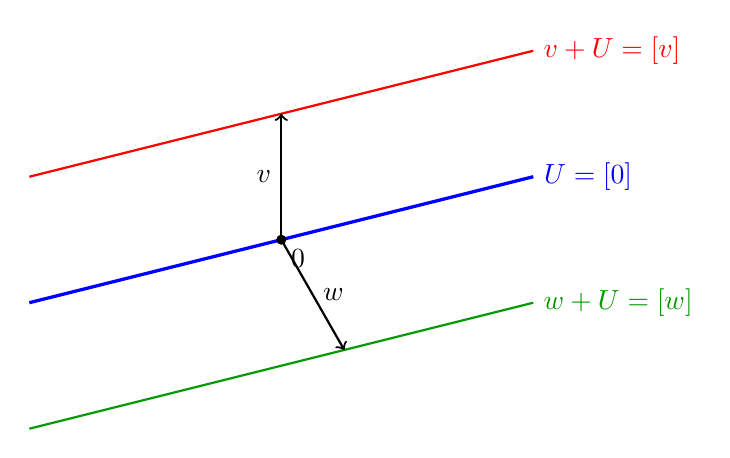
\begin{tikzpicture}[scale=0.8]
    % The subspace U (origin line)
    \draw[very thick, blue] (-4,-1) -- (4,1) node[right] {$U = [0]$};

    % Other equivalence classes (Cosets)
    \draw[thick, red] (-4, 1) -- (4, 3) node[right] {$v + U = [v]$};
    \draw[thick, green!60!black] (-4, -3) -- (4, -1) node[right] {$w + U = [w]$};

    % Vectors defining the shift
    \draw[->, thick] (0,0) -- (0,2) node[midway, left] {$v$};
    \draw[->, thick] (0,0) -- (1,-1.75) node[midway, right] {$w$};

    % Origin
    \filldraw (0,0) circle (2pt) node[below right] {$0$};
  \end{tikzpicture}
\end{center}

\subsection{The Vector Space Structure of $V/U$}

We want to turn $V/U$ into a vector space over $K$. We define addition as $[v_1] + [v_2] := [v_1 + v_2]$ for all $[v_1], [v_2] \in V/U$. Alternatively, this can be written as $(v_1 + U) + (v_2 + U) := (v_1 + v_2) + U$. For scalar multiplication, let $\alpha \in K$ and $[v] \in V/U$. We define $\alpha \cdot [v] := [\alpha v]$. The zero element is defined as $0_{V/U} := [0_V] = U$.

\begin{proposition}[Well-definedness of Operations in $V/U$]
  The operations defined above are well-defined. Moreover, they give $V/U$ the structure of a vector space over $K$.
\end{proposition}

\begin{proof}
  To establish well-definedness, we must show that the operations do not depend on the choice of representatives.
  For scalar multiplication, suppose $[v] = [v']$, and let $\alpha \in K$. We need to show that $[\alpha v] = [\alpha v']$. Indeed, since $[v] = [v']$, we have $v - v' \in U$. Because $U$ is a subspace, $\alpha(v - v') = \alpha v - \alpha v' \in U$. Consequently, $[\alpha v] = [\alpha v']$.

  Similarly, for addition, suppose $[v_1] = [v_1']$ and $[v_2] = [v_2']$. We need to show that $[v_1 + v_2] = [v_1' + v_2']$. By assumption, $v_1 - v_1' \in U$ and $v_2 - v_2' \in U$. Adding these yields:
  \[ (v_1 + v_2) - (v_1' + v_2') = (v_1 - v_1') + (v_2 - v_2') \in U. \]
  Therefore, $v_1 + v_2 \sim v_1' + v_2'$, which implies $[v_1 + v_2] = [v_1' + v_2']$. This proves that the operations are well-defined.

  It remains to show that they satisfy the axioms of a vector space. These follow directly from the corresponding axioms in $V$. (Exercise: complete the proof!)
\end{proof}

We now define a map $\pi \colon V \to V/U$ by $\pi(v) := [v] \in V/U$ for all $v \in V$.

\begin{proposition}[The Quotient Map]
  The map $\pi \colon V \to V/U$ is a linear map. Moreover, it is surjective (i.e., $\operatorname{Im}(\pi) = V/U$), and $\ker(\pi) = U$.
\end{proposition}

\begin{proof}
  Linearity: For $v_1, v_2 \in V$, $\pi(v_1 + v_2) = [v_1 + v_2] = [v_1] + [v_2] = \pi(v_1) + \pi(v_2)$. For $\alpha \in K$ and $v \in V$, $\pi(\alpha v) = [\alpha v] = \alpha [v] = \alpha \pi(v)$.

  Surjectivity: Let $x \in V/U$. By definition, $x$ is an equivalence class $[v]$ of some element $v \in V$. Thus, $x = \pi(v)$.

  Kernel: We claim that $\ker(\pi) = U$. First, let $v \in \ker(\pi)$, meaning $\pi(v) = 0$. Then, $[v] = [0]$, which implies $v = v - 0 \in U$. Hence, $\ker(\pi) \subseteq U$. Conversely, let $u \in U$. Then, $u \sim 0$ because $u - 0 \in U$. Therefore, $\pi(u) = [u] = [0] = 0$, so $u \in \ker(\pi)$. This shows that $U \subseteq \ker(\pi)$, completing the proof.
\end{proof}

\begin{proposition}[Dimension of the Quotient Space]
  Suppose that $V$ is a finite-dimensional vector space. Then, $V/U$ is also finite-dimensional, and $\dim V/U = \dim V - \dim U$.
\end{proposition}

\begin{proof}
  We have seen that $\pi \colon V \to V/U$ is a surjective linear map. This guarantees that $V/U$ is finite-dimensional. (Generally, if $T \colon W' \to W''$ is a surjective linear map and $W'$ is finite-dimensional, then $W''$ is also finite-dimensional, because the images of a basis of $W'$ span $W''$).

  We now apply the Rank-Nullity Theorem to $\pi$:
  \[ \dim V = \dim \ker(\pi) + \dim \operatorname{Im}(\pi). \]
  Since $\ker(\pi) = U$ and $\operatorname{Im}(\pi) = V/U$, we obtain $\dim V/U = \dim V - \dim U$.
\end{proof}

\subsection{The Isomorphism Theorem and Universal Property}

\begin{theorem}[The First Isomorphism Theorem]
  Let $V$ and $W$ be vector spaces over $K$, and let $T \colon V \to W$ be a linear map. We define a new map $\overline{T} \colon V/\ker(T) \to \operatorname{Im}(T)$ as follows: For $x \in V/\ker(T)$, choose a representative $v \in V$ such that $x = [v]$. Define $\overline{T}(x) := T(v)$. Then:
  \begin{enumerate}
    \item $\overline{T}$ is well-defined and is a linear map.
    \item $\overline{T} \colon V/\ker(T) \to \operatorname{Im}(T)$ is an isomorphism.
    \item {The following diagram commutes: $T = i \circ \overline{T} \circ \pi$, where $i \colon \operatorname{Im}(T) \to W$ is the inclusion map.
      \begin{center}
        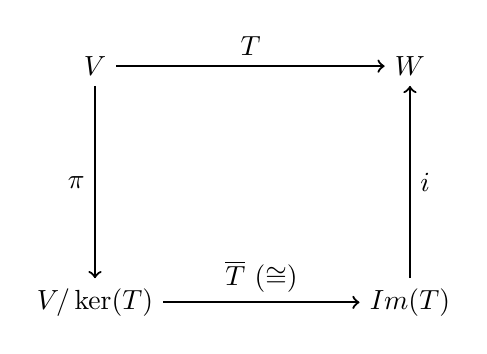
\begin{tikzpicture}[node distance=3cm, auto, thick]
          \node (V) {$V$};
          \node (W) [right of=V, node distance=4cm] {$W$};
          \node (Vmod) [below of=V] {$V/\ker(T)$};
          \node (Im) [below of=W] {$\operatorname{Im}(T)$};

          \draw[->] (V) to node {$T$} (W);
          \draw[->] (V) to node[swap] {$\pi$} (Vmod);
          \draw[->] (Vmod) to node {$\overline{T} \ (\cong)$} (Im);
          \draw[->] (Im) to node[swap] {$i$} (W);
        \end{tikzpicture}
      \end{center}
    }

  \end{enumerate}
\end{theorem}

\begin{proof}
  \begin{enumerate}
    \item To show that $\overline{T}$ is well-defined, suppose $x = [v] = [v']$. We must show that $T(v) = T(v')$. Indeed, $[v] = [v']$ implies that $v - v' \in \ker(T)$, meaning $T(v - v') = 0$. By linearity, $T(v) = T(v')$.

    The linearity of $\overline{T}$ is straightforward: $\overline{T}(\alpha[v]) = \overline{T}([\alpha v]) = T(\alpha v) = \alpha T(v) = \alpha \overline{T}([v])$. Also, $\overline{T}([v_1] + [v_2]) = \overline{T}([v_1 + v_2]) = T(v_1 + v_2) = T(v_1) + T(v_2) = \overline{T}([v_1]) + \overline{T}([v_2])$.

    \item To show that $\overline{T}$ is injective, let $x \in \ker(\overline{T})$, and write $x = [v]$ for some $v \in V$. Then, $\overline{T}(x) = T(v) = 0$, meaning $v \in \ker(T)$. This implies that $x = [v] = 0_{V/\ker(T)}$.

    To show that $\overline{T}$ is surjective, let $w \in \operatorname{Im}(T)$. Then, there exists $v \in V$ such that $T(v) = w$. Consequently, $\overline{T}([v]) = T(v) = w$, proving surjectivity.

    \item The commutativity of the diagram follows immediately from the definitions.
  \end{enumerate}
\end{proof}

\begin{theorem}[Universal Property of Quotient Spaces]
  Let $V$ be a vector space over $K$, and let $U \subseteq V$ be a subspace. The quotient space $V/U$ has the following universal property: For every vector space $W$ and every linear map $T \colon V \to W$ for which $T(U) = 0$ (i.e., for which $\ker(T) \supseteq U$), there exists a unique linear map $T' \colon V/U \to W$ such that $T = T' \circ \pi$. Moreover, $\ker(T') = \ker(T)/U$.
\end{theorem}

\begin{remark}
  In algebraic jargon, every linear map $T \colon V \to W$ that maps $U$ to $0$ factors through $V/U$ via $T = T' \circ \pi$, and moreover, in a unique way. We say that $T$ induces the map $T'$, or that $T$ descends to a map $T' \colon V/U \to W$.
\end{remark}

\begin{proof}
  We define $T' \colon V/U \to W$ as follows: let $x \in V/U$ and choose $v \in V$ such that $x = [v]$. Define $T'(x) := T(v)$. The proof that $T'$ is well-defined and linear follows the exact same logic as in the Isomorphism Theorem. The diagram commutes by construction, since $T'(\pi(v)) = T'([v]) = T(v)$.

  For uniqueness, suppose $T = T'' \circ \pi$ is another factorization. We will show that $T'' = T'$. Let $x \in V/U$. Since $\pi$ is surjective, there exists $v \in V$ such that $x = \pi(v)$. We then have $T(v) = T'(\pi(v))$ and $T(v) = T''(\pi(v))$, which immediately yields $T'(x) = T''(x)$.
\end{proof}

\subsection{Quotients, Complements, and Dual Spaces}

Let $V$ be a vector space over $K$, and let $U \subseteq V$ be a subspace. Let $W \subseteq V$ be a complement of $U$ (i.e., $W$ is a subspace such that $U \cap W = \{0\}$ and $U + W = V$).

\begin{proposition}[Canonical Isomorphism from a Complement]
  Under the assumptions above, there is a canonical isomorphism $Q \colon W \to V/U$, defined by $Q(w) := [w] \in V/U$ for all $w \in W$.
\end{proposition}

\begin{remark}
  The isomorphism $Q$ is canonical only once the complement $W$ is specified. In general, there are many choices of complements to $U$, and there is no preferred choice.
\end{remark}

\begin{proof}
  Consider the inclusion map $i \colon W \to V$ and the projection map $\pi \colon V \to V/U$. Since $Q = \pi \circ i$, $Q$ is a linear map.

  We claim that $\ker(Q) = \{0\}$. Indeed, if $w \in \ker(Q)$, then $[w] = 0$, implying that $w \in U$. However, since $w \in W$, we must have $w \in U \cap W = \{0\}$, and therefore $w = 0$. This shows that $\ker(Q) = \{0\}$.

  We also claim that $Q$ is surjective. Let $x \in V/U$ and choose $v \in V$ such that $x = [v]$. Since $V = U + W$, there exist $u \in U$ and $w \in W$ such that $v = w + u$. It follows that $[v] = [w + u] = [w]$, so $Q(w) = x$. This proves that $Q$ is surjective, and consequently, an isomorphism.
\end{proof}

\subsection{Quotients, Complements, and Annihilators}

\begin{proposition}[Isomorphism from a Specified Complement]
  Let $W \subseteq V$ be a complement of $U$ in $V$. There exists a canonical isomorphism $Q \colon W \to V/U$ defined by $Q(w) := [w]$.
\end{proposition}

\begin{proof}
  $Q$ is the composition of the inclusion $i \colon W \to V$ and the projection $\pi \colon V \to V/U$, and thus is linear. Since $W \cap U = \{0\}$, the kernel of $Q$ is trivial. As $V = U + W$, any $v \in V$ can be written as $w + u$, so $[v] = [w + u] = [w]$, which is $Q(w)$. This proves surjectivity and establishes the isomorphism.
\end{proof}

\begin{proposition}[Annihilators and Dual Quotients]
  Let $U \subseteq V$ be a subspace, and define the annihilator $U^\perp := \{l \in V^* \mid l|_U = 0\}$. Then:
  \begin{enumerate}
    \item $U^\perp \subseteq V^*$ is a linear subspace.
    \item There is a canonical isomorphism $(V/U)^* \cong U^\perp$.
    \item If $V$ is finite-dimensional, then $U^* \cong V^*/U^\perp$.
  \end{enumerate}
\end{proposition}

\begin{proof}
  \begin{enumerate}
    \item Clearly, the zero functional vanishes on $U$. For $l_1, l_2 \in U^\perp$ and $\alpha, \beta \in K$, we have $(\alpha l_1 + \beta l_2)(u) = \alpha l_1(u) + \beta l_2(u) = 0$ for all $u \in U$, establishing that $U^\perp$ is a subspace.

    \item We define a map $L \colon (V/U)^* \to U^\perp$ by $L(s) := s \circ \pi$. This map is well-defined because for any $u \in U$, $(s \circ \pi)(u) = s([u]) = s(0) = 0$. To show linearity, let $s, t \in (V/U)^*$ and $\alpha, \beta \in K$; then
    \[ L(\alpha s + \beta t) = (\alpha s + \beta t) \circ \pi = \alpha(s \circ \pi) + \beta(t \circ \pi) = \alpha L(s) + \beta L(t). \]
    We define an inverse $P \colon U^\perp \to (V/U)^*$ such that for $T \in U^\perp$, $P(T) = T'$, where $T'$ is the unique map induced by the Universal Property of Quotients such that $T = T' \circ \pi$. The identities $L \circ P = \operatorname{id}$ and $P \circ L = \operatorname{id}$ confirm $L$ is a canonical isomorphism.

    \item Assume $V$ is finite-dimensional. Define the restriction map $R \colon V^* \to U^*$ by $R(\varphi) := \varphi|_U$. This map is linear, as $R(\alpha \varphi + \beta \psi) = (\alpha \varphi + \beta \psi)|_U = \alpha R(\varphi) + \beta R(\psi)$. By extending a basis of $U$ to $V$, we can construct a functional on $V$ that matches any functional on $U$, showing $R$ is surjective. Since $\ker(R) = \{\varphi \in V^* \mid \varphi|_U = 0\} = U^\perp$, the First Isomorphism Theorem yields $V^*/U^\perp \cong U^*$.
  \end{enumerate}
\end{proof}

\begin{exercise}
  Let $T \colon V \to W$ be a linear map between vector spaces. Prove that the annihilator of the image of $T$ is equal to the kernel of its dual map:
  \[ (\operatorname{Im} T)^\perp = \ker(T^*). \]
\end{exercise}
